\documentclass[10pt,a4paper]{article}
\usepackage[T1]{fontenc}
\usepackage{lmodern}
\usepackage[a4paper,margin=1.9cm]{geometry}
\usepackage{microtype}
\usepackage{amsmath}
\usepackage{booktabs}
\usepackage{caption}
\usepackage{titlesec}
\usepackage{xcolor}
\usepackage{tikz}
\usetikzlibrary{arrows.meta,positioning}

\titlespacing*{\section}{0pt}{9pt}{3pt}
\titlespacing*{\subsection}{0pt}{6pt}{2pt}
\titleformat{\section}{\large\bfseries}{\thesection.}{0.5em}{}
\titleformat{\subsection}{\normalsize\bfseries}{\thesubsection}{0.5em}{}
\captionsetup{font=small,labelfont=bf,skip=4pt}
\setlength{\parskip}{3pt}
\setlength{\parindent}{0pt}
\newcommand{\code}[1]{\texttt{#1}}

\begin{document}

\begin{center}
{\Large\bfseries Deadline Scheduler with Priority Donation Through Pipes on xv6}\\[4pt]
{\normalsize CSL3030 Operating Systems Lab, IIT Jodhpur \quad$\cdot$\quad Team KernelKraft \quad$\cdot$\quad 11 November 2026}\\[3pt]
{\normalsize Atharv Dhuvad (B24CS1085) \quad Ridham Shah (B24CS1064) \quad Pranav H Nair (B24CS1056)}
\end{center}
\vspace{-4pt}\hrule\vspace{4pt}

\section{Problem}

A pipeline is only as fast as its slowest stage. If the last stage of a pipeline has a deadline but the stages feeding it do not, an earliest-deadline-first (EDF) scheduler treats those earlier stages exactly like any unrelated CPU-bound process. The urgent stage will then sleep on an empty pipe while the process that should fill it waits its turn due to a running CPU hog. This is priority inversion, and simple EDF does not solve it. Our project replaces the xv6 round-robin scheduler with EDF and removes the inversion by letting a blocked reader pass its deadline to the writer of the pipe it is waiting on.

\section{Implementation}

\subsection{Workflows and the EDF scheduler}

The system call \code{setworkflow(wid, D)} places the calling process in workflow \code{wid}. The first caller fixes the workflow's absolute deadline at $\textit{now} + D$ ticks. Every later caller joins the same workflow and takes that deadline, so all members share it regardless of when they call, and a child created by \code{fork} inherits it. A process outside any workflow has deadline $\infty$. Each process stores two fields, its own deadline $d_{\text{own}}$ and a donated deadline $d_{\text{don}}$, and the scheduler orders processes by
\[
d_{\text{eff}}(p) \;=\; \min\bigl(d_{\text{own}}(p),\; d_{\text{don}}(p)\bigr).
\]
Keeping the donated value in a separate field means a donation can be withdrawn without losing the process's own deadline. On every scheduling decision the kernel scans the process table under \code{ptable.lock} and runs the runnable process with the smallest $d_{\text{eff}}$. Deadlines are compared with a signed difference so that the order survives wrap-around of the tick counter, and ties are broken in favour of the process that ran least recently, which makes processes without deadlines share the CPU fairly. The kernel boots in default with EDF with donation. Round-robin and plain EDF are selectable at run time through \code{setsched} so that all three policies can be measured on the same kernel.

\subsection{Donation through pipes}

\begin{figure}[h]
\centering
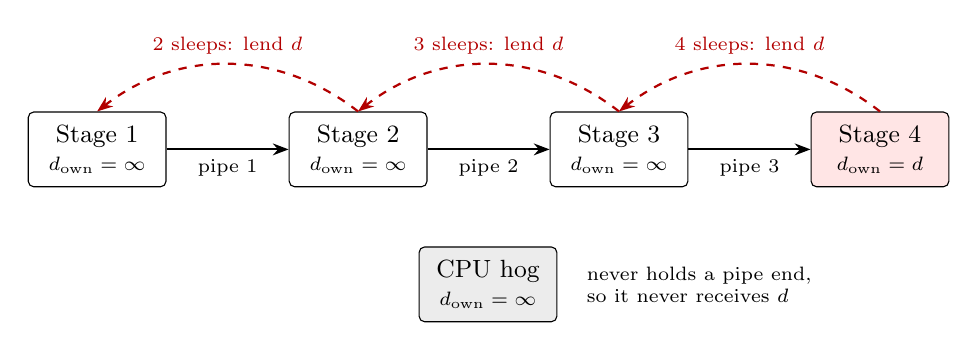
\begin{tikzpicture}[
  node distance=1.55cm,
  stage/.style={draw,rounded corners=2pt,minimum width=1.75cm,minimum height=0.95cm,align=center,font=\small},
  data/.style={-{Stealth[length=2mm]},thick},
  don/.style={-{Stealth[length=2mm]},thick,dashed,red!70!black},
  lab/.style={font=\scriptsize}]
\node[stage] (s1) {Stage 1\\[-1pt]\scriptsize $d_{\text{own}}=\infty$};
\node[stage,right=of s1] (s2) {Stage 2\\[-1pt]\scriptsize $d_{\text{own}}=\infty$};
\node[stage,right=of s2] (s3) {Stage 3\\[-1pt]\scriptsize $d_{\text{own}}=\infty$};
\node[stage,right=of s3,fill=red!10] (s4) {Stage 4\\[-1pt]\scriptsize $d_{\text{own}}=d$};
\node[stage,below=0.75cm of s2,xshift=1.65cm,fill=gray!15] (hog) {CPU hog\\[-1pt]\scriptsize $d_{\text{own}}=\infty$};
\draw[data] (s1.east) -- node[lab,below]{pipe 1} (s2.west);
\draw[data] (s2.east) -- node[lab,below]{pipe 2} (s3.west);
\draw[data] (s3.east) -- node[lab,below]{pipe 3} (s4.west);
\draw[don] (s4.north) to[bend right=38] node[lab,above]{4 sleeps: lend $d$} (s3.north);
\draw[don] (s3.north) to[bend right=38] node[lab,above]{3 sleeps: lend $d$} (s2.north);
\draw[don] (s2.north) to[bend right=38] node[lab,above]{2 sleeps: lend $d$} (s1.north);
\node[lab,right=0.25cm of hog,align=left] {never holds a pipe end,\\so it never receives $d$};
\end{tikzpicture}
\caption{Data flows left to right through the pipes (solid). When a reader sleeps on an empty pipe, its effective deadline flows right to left to the writer (dashed), and continues backwards if that writer is itself asleep on a pipe. Every stage then outranks the hog.}
\label{fig:donation}
\end{figure}

Figure~\ref{fig:donation} shows the mechanism. Just before \code{piperead} puts a process to sleep on an empty pipe, the kernel records which pipe it is waiting on. If the process has a finite effective deadline, the kernel lowers $d_{\text{don}}$ of the pipe's writer to that deadline. If the writer is itself asleep on another pipe, the same deadline is passed to that pipe's writer, and so on along the chain.

\textbf{Choosing the receiver.} \code{struct pipe} records its writer side: the last process that wrote to it. If that process still holds the write end, then, only that process receives the donation. A first read usually blocks before anything has been written, when no writer is known yet. In that case every process that holds the write end receives the donation, because any of them may be the one that fills the pipe.

\textbf{Chains and cycles.} The walk along the chain is an iterative depth first search with an explicit stack, which will always be bounded by the size of the process table, so it uses a fixed amount of kernel stack and can't run forever. Processes along the current path are flagged. Encountering a flagged process indicates a deadlock: two processes are each waiting on a pipe the other must fill. The kernel notes this and doesn't follow that edge.

\textbf{Withdrawal.} A donation must end when the pipe receives data, when the reader exits, and when the donor is killed. Instead of keeping a list of donors per process, we clear every donated field and rebuild them all from the readers that are still asleep, repeating until nothing changes. If two readers have lent to the same writer and one is killed, the rebuild restores the other's deadline automatically, with no list to maintain.

\textbf{Fork.} Donation is decided when a reader goes to sleep, so a writer created afterwards would be missed. \code{fork} therefore checks whether the child inherits the write end of a pipe that an urgent reader is already asleep on, and donates to the child if so.

All of this runs under the single \code{ptable.lock}, always taken after the pipe's own lock, and diagnostic printing is deferred until the lock has been released. A print mode (\code{tracectl 3}) logs each donation as \code{donate: donor=19 recv=18 dl=725}.

\section{Evaluation}

The workload generator \code{wfgen} builds a pipeline of 2 to 6 stages in which only the final stage joins a workflow, alongside a chosen number of CPU hogs. We measured a 4-stage pipeline moving 2048 bytes, four times the pipe buffer, so that every stage really blocks. Its unloaded completion time on one CPU is $W = 48.2$ ticks, and the deadline is $D = \operatorname{round}(\alpha W)$. Each cell is 20 fresh boots of QEMU, with 3 hogs on one CPU and 8 hogs on three CPUs.

\begin{table}[h]
\centering
\small
\begin{tabular}{@{}cc ccc c ccc@{}}
\toprule
 & & \multicolumn{3}{c}{1 CPU, 3 hogs} & & \multicolumn{3}{c}{3 CPUs, 8 hogs} \\
\cmidrule(lr){3-5}\cmidrule(l){7-9}
$\alpha$ & $D$ (ticks) & RR & EDF & EDF + donation & & RR & EDF & EDF + donation \\
\midrule
1.2 & 58  & 20 & 20 & \textbf{2} & & 20 & 20 & \textbf{10} \\
1.5 & 72  & 20 & 20 & \textbf{1} & & 18 & 20 & \textbf{8} \\
2.0 & 96  & 1  & 5  & \textbf{0} & & 2  & 0  & \textbf{0} \\
3.0 & 145 & 0  & 0  & \textbf{0} & & 0  & 0  & \textbf{0} \\
\midrule
\multicolumn{2}{@{}l}{Mean finish (ticks, 80 runs)} & 96.7 & 96.3 & \textbf{55.9} & & 84.7 & 81.2 & \textbf{67.6} \\
\bottomrule
\end{tabular}
\caption{Deadline misses out of 20 runs per cell, and mean pipeline completion time over all 80 runs of each policy and CPU count. All 480 runs are from one kernel commit and completed with status \code{ok}.}
\label{tab:results}
\end{table}

Table~\ref{tab:results} gives the outcome. Plain EDF is no better than round-robin: the only process with a deadline spends its time asleep, so EDF has nothing urgent to run and the earlier stages share the CPU with the hogs. With donation on one CPU the pipeline finishes in about 56 ticks, not far above its unloaded 48, against about 96 ticks for the other two policies, and misses 1 of 20 deadlines at $\alpha = 1.5$ whereas they miss all 20. On three CPUs donation never misses more often than either baseline, and misses 8 of 20 at $\alpha = 1.5$ against 18 and 20. The gain is smaller there for a reason explained under Limits in Section~5. Comparing EDF with and without donation at $\alpha = 1.5$, Fisher's exact test gives $p = 3.0 \times 10^{-10}$ on one CPU and $p = 4.5 \times 10^{-5}$ on three. With generous deadlines ($\alpha = 3$) no policy misses, as expected.

Correctness was checked separately. \code{donate5} runs a 5-stage chain against a hog and shows the deadline hopping back across all four pipes. \code{cycletest} builds a two-process pipe cycle; the kernel prints \code{donate: cycle} and keeps running on one and three CPUs. \code{killtest} kills two donors in turn and checks that the receiver keeps the deadline after the first kill and loses it after the second. The stock \code{usertests} suite passes under the new scheduler.

\section{Challenges}

\textbf{An unset donation that looked urgent.} ``No donation'' is stored as \code{0xffffffff}. Under the wrap-safe signed comparison that value behaves like $-1$, the earliest possible deadline, so in our first pilot EDF and EDF with donation both finished about 30 ticks late. The fix was to test for the sentinel before comparing.

\textbf{A refused workflow that blocked its identifier.} A GDB session at a breakpoint in \code{setworkflow} showed that a request refused by admission control still left its table slot marked in use with zero members. Nothing ever freed it, so every later request for that workflow was refused too. The table is now written only after admission succeeds, and the same session on the fixed kernel shows the slot staying empty.

\textbf{Blocking before the writer exists.} On three CPUs the cycle test printed no cycle. A reader had gone to sleep before the other process was forked, so the donation walk never saw it. This led to the \code{fork} check described above.

\textbf{Measuring the right thing.} Our first batch of measurements moved fewer bytes than the pipe buffer holds, so stages rarely blocked and donation was rarely exercised. We archived that batch and repeated it with a larger payload. On three CPUs, five hogs were not enough to load the machine and all three policies met every deadline, so we raised the load to eight hogs and repeated the full sweep on the final kernel. xv6 also started only one CPU on the default QEMU machine type until we selected an older one.

\section{Design choices we consider our own}

\textbf{Recomputing instead of bookkeeping.} Rebuilding all donations from the set of sleeping readers costs a bounded scan of the process table, but it makes withdrawal with several donors correct by construction, where a donor list would need careful updates on every wake-up, exit and kill.

\textbf{A recorded writer with a safe fallback.} Recording one writer per pipe is simple but is wrong before the first write. Donating to every holder of the write end is always safe but can boost a process that merely kept a descriptor open. We use the recorded writer when it is valid and fall back to the holders only when it is not.

\textbf{Firm deadlines and admission.} Once a process has missed, its own deadline stops counting, so late work cannot starve work that can still finish on time. The kernel also refuses a new workflow whose deadline is under 20 ticks away, since it could not be met.

\textbf{Evidence we can trust.} We committed written predictions to the repository before running our measurement batch of 6 November, and every row of results carries the commit hash of the kernel that produced it and the path of its raw QEMU log.

\textbf{Limits.} A donation lasts only while the reader is asleep, as the problem statement requires. On one CPU that is almost always the case. On three CPUs the reader often runs at the same time as its writer, and each time it wakes the writer drops back to competing with the hogs until the reader sleeps again. This is why donation still misses some tight deadlines on three CPUs in Table~\ref{tab:results}. The recomputation is also quadratic in the number of processes, which is acceptable for the 64 that xv6 allows.

\end{document}
